\newpage
\section{Resultados}

\subsection{Atividade 1 – Circuitos Ressonantes}

Para o circuito ressonante da figura \ref{fig:Qload}, primeiramente calculamos 
a frequência de ressonância, como mostrado abaixo:

\[
  f_0 = \frac{1}{2 \pi \sqrt{LC}} = \frac{1}{2 \pi \sqrt{2.10^{-6} \times 
  22.10^{-9}}} = 758,54kHz.
\]

A frequência de ressonância medida foi muito próxima da frequência de 
ressonância calculada, tendo um valor de 758,57 kHz.
Para a frequência de ressonância analisada no gráfico, observamos uma tensão de 
pico correspondente a 903,84 mV.

\begin{figure}[H]
  \centering
  \caption{Sinal da função de transferência para um circuito ressonante 
  paralelo.}
  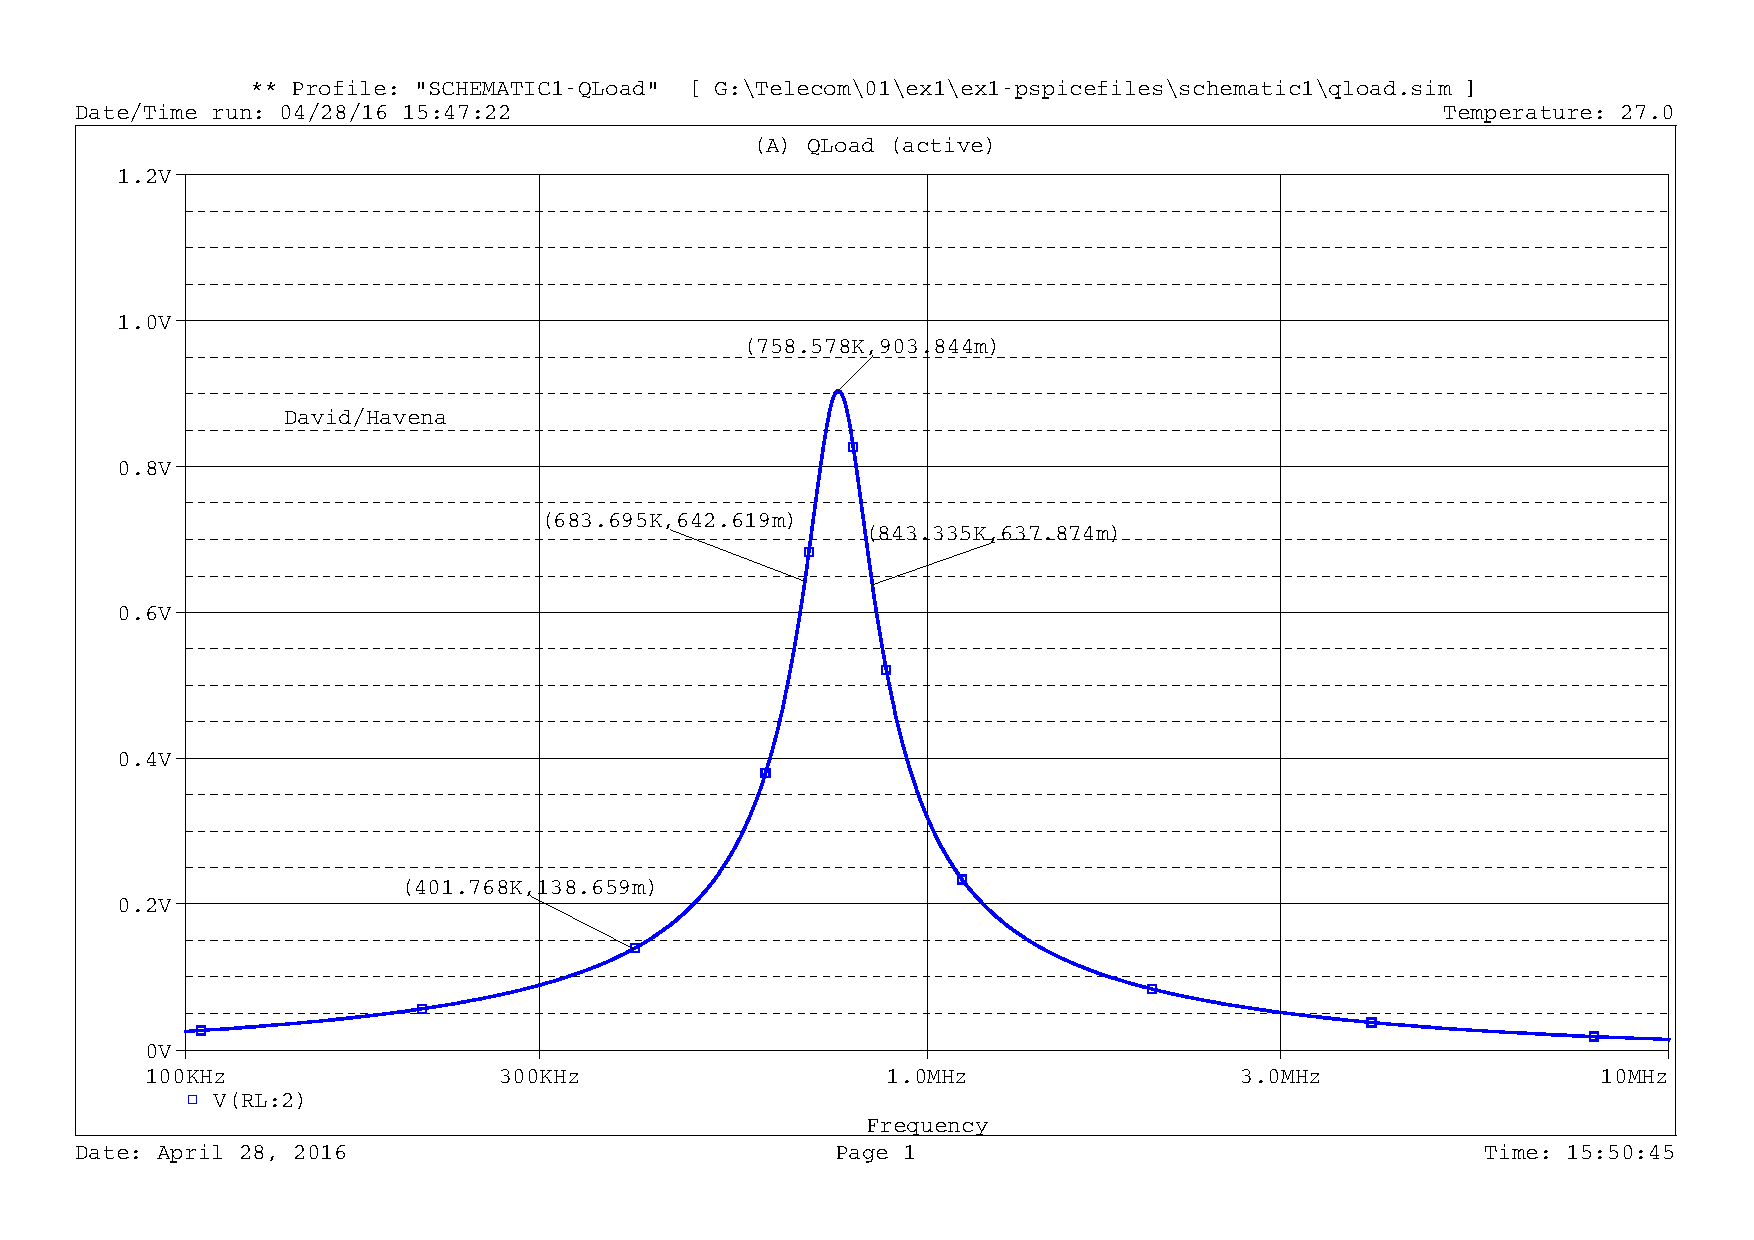
\includegraphics[scale=0.5]{05.pdf}
  
  \label{fig:Qload}
\end{figure}

A tensão de largura de banda foi calculada, utilizando-se a tensão de pico 
correspondente a frequência de ressonância, como mostrado abaixo:
